\chapter{Runtime View (Dynamic View)}

\section{System Initialization}
SUSD has an initialization routine, invoked by the BSW.

\Requirement{019}
{\Function{SUSD_Init}
{\code{void}}{}{}
{\code{void}}
{SUSD sets the application state manager state to Init when this function is invoked.}
}
{\Satisfies{SRS_SUSD 001} \Satisfies{SRS_SUSD 052} \Satisfies{SRS_SUSD 129} \Satisfies{SRS_SUSD 004}}

\section{System De-initialization}
N/A

\section{Detailed Design}
\label{sec:detaileddesign}
\begin{enumerate}
\item The common interfaces among SUMs and SWCs are defined in \file{GM_SUM_Interfaces.arxml}.
\item \Requirement{133}{Permit Execution Interface with SUM_PNC, SUM_LNM, SUM_ERRH and SUM_SOH shall follow the order of invoking as mentioned, remaining SUMs shall be invoked after SUM_SOH in any order.}
{\Satisfies{SRS_SUSD 002}}
\item \Requirement{134}{The disabling of PermitExecution of SUMs from SUM_SUSD shall follow this order: SUM_SOH, SUM_ERRH, SUM_LNM, SUM_PNC.}
{\Satisfies{SRS_SUSD 003}}
\item Shutdown Permission interface shall be with SUM_PNC, SUM_LNM, SUM_SSFM-ERRH, SUM_SOH, SUM_DIAG, SUM_SSC, SUM_SSFM-SSM, SUM_TCS, SUM_SrvcMgr and SUM_SPM.
\end{enumerate}

\subsection{Macros}
\label{sec:macros}

\Requirement{102}
{\Macro{ENABLESHUTDOWN}
{255}
{Value received from individual SW-C to enable shut down.}}
{\Satisfies{SRS_SUSD 261}}

\Requirement{103}
{\Macro{SUSD_CONTROLLER_VOLTAGE_THRESHOLD}
{95u}
{Controller Voltage Threshold with a resolution of 100 mV.}}
{\Satisfies{SRS_SUSD 194}\Satisfies{SRS_SUSD 229}}

\Requirement{104}
{\Macro{SUSD_CONTROLLER_VOLTAGE_HYSTERESIS_LOW}
{5u}
{Controller Voltage Hysteresis when going low, with a resolution of 100 mV.}}
{\Satisfies{SRS_SUSD 194} \Satisfies{SRS_SUSD 229}}

\subsection{Data Types}


\Requirement{135}
{
\Datatype{SUSD_SWC_ExecutionStatusType}
{\code{uint8}}
{Notification from SUSD to individual SW-Cs to execute their features based on the correct combination of wakeups, vehicle power mode, battery voltage, etc.

Bit values: 
\begin{description}
\item[0] Wakeup(s) relevant to this SW-C active (0: False, 1: True)
\item[1] Shutdown target bit (0: OFF, 1: NOT\_OFF)
\item[2] HW peripheral(s) relevant to this SW-C	0 initialized (0: False, 1: True)
\item[3] Vehicle Power Mode relevant to this SW-C in an operational state (0: False, 1: True)
\item[4] Reserved for future use by SUSD (set to 0)
\item[5] Battery Voltage Level relevant to this SW-C active (0: False, 1: True)
\item[6] ECU Reset Requested (0: True, 1: False)
\item[7] Reserved for future use by SUSD (Set to 0)
\end{description}
}
}
{\Satisfies{SRS_SUSD 098} \Satisfies{SRS_SUSD 055} \Satisfies{SRS_SUSD 056} \Satisfies{SRS_SUSD 101}}

\Requirement{136}
{
\Datatype{SUSD_UserRequestType}
{\code{uint8}}
{Enable from individual SW-C to SUSD to shut down. SUSD will request shutdown to BswM when all SW-C are sending EnableShutdown.

Ranges: 
\begin{description}
\item[0 - 3] DisableShutdown: aliveness rolling count from 0 to 3. Wrap around to 0. SWC needs SUSD to keep the ECU alive so that it can execute its features.
\item[4 - 253] Reserved for future use by SUSD
\item[254] SPM\_Shutdown\_Ready: valid only for SUM\_SPM to indicate that shutdown preconditions inside SPM are fulfilled.
\item[255] EnableShutdown: SW-C has no more need to keep the ECU alive.
\end{description}
}
}
{\Satisfies{SRS_SUSD 099} \Satisfies{SRS_SUSD 102}}

\Requirement{137}
{
\Datatype{CurrentECUOperatingModeType}
{\code{uint8}}
{These are the states of the Application State Manager sub function of SUM_SUSD:

\begin{description}
\item[0: SUM_INIT] Initial state until Application State Manager completes initialization.
\item[1: SUM_RUN] Next state after initialization. In this state, SUM_SUSD is requesting BswM to keep the BSW in the RUN state.
\item[2: SUM_SLEEP] Low Power state requested. ONLY for ECUs which have project specific HW designs which can detect their own wakeups in all vehicle power modes
\item[3: SUM_RESET] Reset the ECU requested.
\item[4: SUM_BOOT] Reprogramming request from diagnostic tool successfully received and all SW-C have voted for shutdown.
\item[5: SUM_SHUTDOWN] Perform ECU Shutdown process, for ECUs that may not support retained power w.r.t memory content.
\end{description}
}
}
{\Satisfies{SRS_SUSD 100} \Satisfies{SRS_SUSD 022} \Satisfies{SRS_SUSD 103}}


\Datatype{SUSD_SOH_ResetOccurredType}
{\code{uint8}}
{SUM_SUSD will send notification to SUM_SOH regarding the occurrence of a reset event and the type of the reset event.

Ranges: 
\begin{description}
\item[0x00] default value.
\item[0x01] Delayed Reset occurred.
\item[0x02] Immediate Reset occurred.
\item[0x03 - 0xFF] Invalid.
\end{description}
}

\subsection{Structures}

\Struct{SUSD_SWCRteInterfaces}
{\begin{itemize}
\item Pointer to Permit Execution interface, mapping of SWC with the wakeup to indicate the Permit Execution.
\item Pointer to Shutdown Permission interface, mapping of SWC with the wakeup to read the Shutdown Permission.
\item Pointer to ShutdownPermControl, the boolean calibration parameter for each shutdown permission interface to control the processing of its permissions.
\end{itemize}}
{Structure to map the interfaces for SW-C.}

\Struct{SUSD_SWCToVoltRangeReferenceType}
{\begin{itemize}
\item Pointer to Permit Execution interface, mapping of SWC with the wakeup to indicate the Permit Execution.
\item Index of a SW-C in a list of configured SW-Cs which are sorted by SUSD_SWCName.
\end{itemize}}
{Structure to map a battery voltage range to its SWCs}

\Struct{SUSD_BatteryVoltageRangeType}
{\begin{itemize}
\item Pointer to Battery Voltage Min to Max, the mapping of SWC with the limit for normal/over/under voltage to indicate same to respective SW-C.
\item Pointer to SWC_UnderVoltageHysteresis, the calibration value for Under Voltage Limit for specific SW-C.
\item Pointer to SWC_OverVoltageHysteresis, the calibration value for Over Voltage Limit for specific SW-C.
\item The minimum voltage in range.
\item The maximum voltage in range.
\item Number of SWC refer to the range.
\item Pointer to the mapping between SW-Cs and a voltage range.
\end{itemize}}
{Structure of a configured battery voltage range}


\subsection{Enums}

\Requirement{105}
{\Enum{SUSD_DiagnosticStatusType}
{\begin{description}
\item[0x00: SUSD_DIAGNOSTIC_NO_STATUS_TO_REPORT] Run Crank Input Stuck High/Low Diagnostic is not presently being set to Passed nor Failed.
\item[0x01: SUSD_DIAGNOSTIC_PASSED] Run Crank Input Stuck High/Low Diagnostic has passed.
\item[0x02: SUSD_DIAGNOSTIC_FAILED] Run Crank Input Stuck High/Low Diagnostic has failed.
\end{description}}
{Enumeration values for Run Crank Input Stuck High/Low Diagnostic Status.}}
{\Satisfies{SRS_SUSD 190} \Satisfies{SRS_SUSD 225} \Satisfies{SRS_SUSD 191}}

\section{Shutdown permission and timers}

SUSD manages the Shutdown Permission mechanism using two classes of timers:

\begin{itemize}
\item Per-component refresh timers (array): for each \emph{ShutdownPermission} interface SUSD maintains a refresh timer. Each SW-C exposing a \emph{ShutdownPermission} shall periodically send a refresh within the interval configured by the parameter \textbf{SUSD\_t\_Shoutdown\_Refresh}. A refresh resets the corresponding timer; if the timer expires the component's permission is considered invalid.
\item Global force-shutdown timer: when no component has an active \emph{PermitExecution}, SUSD starts a global timer configured by the parameter \textbf{SUSD\_t\_Force\_shutdown\_Wait}. When this timer expires SUSD requests BswM to transition to Shutdown.
\end{itemize}

Operational behaviour:
\begin{itemize}
\item SUSD internal state is updated when a local refresh timer expires: the component loses the ability to grant shutdown permission until a new refresh is received.
\item The global timer is started only when all \emph{PermitExecution} are inactive; if at least one \emph{PermitExecution} becomes active during the global countdown the global timer is cancelled.
\item Internal identifiers used in the implementation may be represented as an array \texttt{SUSD_ShutdownRefreshTimers[]} and a single value \texttt{SUSD_GlobalForceShutdownTimer}, whose intervals are configurable via the parameters above.
\end{itemize}

\section{SPM shutdown sequencing}
SUSD shall manage shutdown signaling for SUM\_SPM with a dedicated sequence based on \code{SUSD\_UserRequestType} and internal vote counters.

\begin{enumerate}
\item When SUSD receives \code{EnableShutdown} (\code{255}) from all required modules on \code{SUSD\_UserRequestType} (SWCs and SUMs, including SUM\_SPM), SUSD may prepare the SPM shutdown path while ignoring SUM\_SSC vote state.
\item SUSD shall evaluate \texttt{GblSUMshutdownenablecnt} and \texttt{Gblshutdownenablecnt} as follows:
\begin{itemize}
\item all required module bits shall be set to 1 (equivalent to \code{0xFF}) in \texttt{Gblshutdownenablecnt};
\item for \texttt{GblSUMshutdownenablecnt}, all SUM bits except SUM\_SSC shall be set to 1 (SUM\_SSC may be either 0 or 1).
\end{itemize}
\item If the condition above is true, SUSD shall set the Shutdown Target bit (bit 1) to OFF (0) in \code{SUSD\_SWC\_ExecutionStatusType} for SUM\_SPM via \texttt{SUSD\_GaaSUMPermitExecution[SUM\_SPM], Shutdown Target bit to 1 (NOT\_OFF)}.
\item For the final ECU shutdown request, SUSD shall additionally require SUM\_SPM to send \code{0xFE} (SPM\_Shutdown\_Ready) on \code{SUSD\_UserRequestType}. Only in this case, and when all other required modules vote \code{EnableShutdown}, SUSD can proceed with the EcuM shutdown request.
\end{enumerate}

\section{Wakeup procedure}
When a wakeup from sleep or battery connect occurs, EcuM validates the wakeup and, if valid, informs BswM, initializes a configurable set of BSWs, and then hands over control to BswM once initialization is complete.
BswM is configured to finish initialization by starting the Schedule Manager and RTE (and any other configured BSW not initialized by EcuM).
At this point the ECU can execute its application SW-Cs.

\section{Sleep procedure}
\Requirement{145}
{BswM does not have any AUTOSAR defined function to determine when the ECU needs to transition to the Shutdown Target (Sleep, Off, or Reset).
It requires an SW-C or BSW to issue a mode request in order to perform any action list which can initiate a shutdown sequence.
The Application State Manager function of SUM_SUSD is responsible for implementing this decision, based on receiving notifications from project specific SW-C via the \code{<SUM/SWC>_SUSD_ShutdownPermission} interface.
Once SUM_SUSD determines that a shutdown of the ECU is required, it issues the corresponding mode request to BswM, which checks the configurable rule, and then (if arbitration is granted) performs the action list containing the shutdown sequence.
One item in the action list will switch the EcuM_State to shut down. When this is done, EcuM will configure the ECU to the Shutdown Target.}
{\Satisfies{SRS_SUSD 016}}


%\section{Boot loading procedure}
%N/A

%\section{Failure handling strategy}
%N/A

\section{Critical timing constraints}
Runnable \RunnableRef{RE_SUSD_AppStateManager} to be given priority among runnables as it contains permit execution and shutdown permission which is needed for other functionalities in SUM SUSD.

\section{Task management}

\subsection{Periodic Runnables}
\label{sec:periodic_runnables}

\Requirement{034}
{\Runnable{RE_SUSD_BatteryNotifications}
{Fixed}
{}
{VehicleBatteryVoltage}
{BatteryVoltage_Actual

BatteryVoltage_DisableNVMWrite}
{}
{\code{void}}
{This runnable is responsible for monitoring the vehicles battery voltage and state of charge, and notify the SW-Cs with the correct current state at the rate \ConfigurationParameterRef{SUSD_t_Battery_Periodicity}.
}}
{\Satisfies{SRS_SUSD 026} \Satisfies{SRS_SUSD 027} \Satisfies{SRS_SUSD 030} \Satisfies{SRS_SUSD 110} \Satisfies{SRS_SUSD 038} \Satisfies{SRS_SUSD 105}}

\Requirement{035}
{\Runnable{RE_SUSD_AppStateManager}
{Fixed}
{}
{SUSD_SOH_ResetOccurred}
{}
{}
{\code{void}}
{This runnable is responsible for managing the startup/shutdown notifications to the SW-Cs based on the input status processed by the runnable at the rate \ConfigurationParameterRef{SUSD_t_AppManager_Periodicity}.
}}
{\Satisfies{SRS_SUSD 009} \Satisfies{SRS_SUSD 010} \Satisfies{SRS_SUSD 004}}

\Requirement{036}
{\Runnable{RE_SUSD_VehiclePowerMode}
{Fixed}
{}
{SystemBackupPowerMode_Av

SystemBackupPowerMode_FsFA

SystemBackupPowerMode_FcFA

SystemBackupPowerMode_FxFA

SystemBackupPowerMode_FsI

SystemBackupPowerMode_FcI

SystemBackupPowerMode_FxI

SystemBackupPowerMode

SystemPowerMode_Av

SystemPowerMode_FsFA

SystemPowerMode_FcFA

SystemPowerMode_FxFA

SystemPowerMode_FsI

SystemPowerMode_FcI

SystemPowerMode_FxI

SystemPowerMode

SystemPowerMode_BackupPowerMode_Av

SystemPowerMode_BackupPowerMode_FsFA

SystemPowerMode_BackupPowerMode_FcFA

SystemPowerMode_BackupPowerMode_FxFA

SystemPowerMode_BackupPowerMode_FsI

SystemPowerMode_BackupPowerMode_FcI

SystemPowerMode_BackupPowerMode_FxI

PrimaryPowerMode_BackupPowerMode}
{NvMService_VehPowerMode

VehiclePowerMode

VehiclePowerMode_Inv}
{Rte_Pim_VehiclePowerMode_State}
{\code{void}}
{This runnable is responsible for managing the Power Mode Slave and has periodicity \ConfigurationParameterRef{SUSD_t_VehiclePowerMode_Periodicity}.
}}
{\Satisfies{SRS_SUSD 011} \Satisfies{SRS_SUSD 127} \Satisfies{SRS_SUSD 073} \Satisfies{SRS_SUSD 074} \Satisfies{SRS_SUSD 124} \Satisfies{SRS_SUSD 126}}

\Requirement{037}
{\Runnable{RE_SUSD_RunCrankManagement}
{Fixed}
{}
{RunCrankInputDiscreteActive

RunCrankInputPercentage

RunCrankInputStuckLow_FA_StatusRequest

RunCrankInputStuckHigh_FA_StatusRequest

SecondaryRunCrankCmdActive_Av

SecondaryRunCrankCmdActive_Inv

SecondaryRunCrankCmdActive_FoFA

SecondaryRunCrankCmdActive_FoI

SecondaryRunCrankCmdActive

PrimaryRunCrankCmdActive_Av

PrimaryRunCrankCmdActive_Inv

PrimaryRunCrankCmdActive_FoFA

PrimaryRunCrankCmdActive_FoI

PrimaryRunCrankCmdActive}
{RunCrankInput

RunCrankInputStuckLowDiag_FA

RunCrankInputStuckHighDiag_FA

RunCrankInput_Inv

RunCrankActive

RunCrankActive_Inv

RunCrankInputStuckHighDiagStatus

RunCrankInputStuckLowDiagStatus}
{}
{\code{void}}
{This runnable is responsible for managing the Run Crank Plausibility with periodicity \ConfigurationParameterRef{SUSD_t_RunCrank_Periodicity}.}
}
{\Satisfies{SRS_SUSD 071} \Satisfies{SRS_SUSD 079} \Satisfies{SRS_SUSD 080}}

\clearpage

\subsection{Triggered Runnables}
\label{sec:Runnable}
\Requirement{039}
{\Runnable{RE_SUSD_DiagnosticReprogrammingRequest}
{Event}
{}{}{}{}
{\code{void}}
{Runnable to be triggered every time there is RTE write from BswM to SUSD on Reprogramming request.}
}
{\Satisfies{SRS_SUSD 013} \Satisfies{SRS_SUSD 108}}

\Requirement{040}
{\Runnable{RE_SUSD_DiagnosticResetRequest}
{Event}
{}{}{}{}
{\code{void}}
{Runnable to be triggered every time there is RTE write from BswM to SUSD on Reset request.}
}
{\Satisfies{SRS_SUSD 014} \Satisfies{SRS_SUSD 107}}

\Requirement{041}
{\Runnable{RE_SUSD_VPwrSetEnableCond}
{Event}
{}{}{}{}
{\code{void}}
{Runnable for Vehicle power mode condition.}
}
{\Satisfies{SRS_SUSD 075}}

\Requirement{042}
{\Function{SUSD_ECU_Operating_State_CheckRead}
{\code{Dcm_OpStatusType OpStatus}: status of the current operation}
{\code{Dcm_NegativeResponseCodeType *ErrorCode}: NRC to be sent in the negative response in case of failure.}
{}
{Std_ReturnType}
{Function for Condition Check Read of ECU Operating State through DID.}
}
{\Satisfies{SRS_SUSD 008}}

\Requirement{043}
{\Function{SUSD_Dcm_ECU_Operating_State}
{\code{Dcm_OpStatusType OpStatus}: status of the current operation.}
{\code{uint8 *Data}: Buffer where ECU Operating State is copied.}
{}
{Std_ReturnType}
{Function for reading ECU Operating State through DID.}
}
{\Satisfies{SRS_SUSD 008}}

\Requirement{046}
{\Function{SUSD_Battery_Voltage_CheckRead}
{\code{Dcm_OpStatusType OpStatus}: status of the current operation}
{\code{Dcm_NegativeResponseCodeType *ErrorCode}: NRC to be sent in the negative response in case of failure.}
{}
{Std_ReturnType}
{Function for Condition Check Read of Battery Voltage Value through DID.}
}
{\Satisfies{SRS_SUSD 025}}

\Requirement{047}
{\Function{SUSD_Dcm_Battery_Voltage}
{\code{Dcm_OpStatusType OpStatus}: status of the current operation.}
{\code{uint8 *Data}: Buffer where Battery Voltage Value is copied.}
{}
{Std_ReturnType}
{Function for Battery Voltage Value through DID.}
}
{\Satisfies{SRS_SUSD 025}}

\Requirement{048}
{\Function{SUSD_Wakeup_Source_Reason_CheckRead}
{\code{Dcm_OpStatusType OpStatus}: status of the current operation}
{\code{Dcm_NegativeResponseCodeType *ErrorCode}: NRC to be sent in the negative response in case of failure.}
{}
{Std_ReturnType}
{Function for Condition Check Read of Wakeup reason through DID.}
}
{\Satisfies{SRS_SUSD 060}}

\Requirement{049}
{\Function{SUSD_Dcm_Wakeup_Source_Reason}
{\code{Dcm_OpStatusType OpStatus}: status of the current operation.}
{\code{uint8 *Data}: Buffer where Wakeup Reason is copied.}
{}
{Std_ReturnType}
{Function for Wakeup reason through DID.}
}
{\Satisfies{SRS_SUSD 060} \Satisfies{SRS_SUSD 053}}

\Requirement{050}
{\Function{SUSD_Active_Wakeup_Sources_CheckRead}
{\code{Dcm_OpStatusType OpStatus}: status of the current operation}
{\code{Dcm_NegativeResponseCodeType *ErrorCode}: NRC to be sent in the negative response in case of failure.}
{}
{Std_ReturnType}
{Function for Condition Check Read of active wakeup sources through DID.}
}
{\Satisfies{SRS_SUSD 060}}

\Requirement{051}
{\Function{SUSD_Dcm_Active_Wakeup_Sources}
{\code{Dcm_OpStatusType OpStatus}: status of the current operation.}
{\code{uint8 *Data}: Buffer where Active Wakeup Source is copied.}
{}
{Std_ReturnType}
{Function for active wakeup sources through DID.}
}
{\Satisfies{SRS_SUSD 060}}

\Requirement{054}
{\Function{SUSD_Power_Moding_State_CheckRead}
{\code{Dcm_OpStatusType OpStatus}: status of the current operation}
{\code{Dcm_NegativeResponseCodeType *ErrorCode}: NRC to be sent in the negative response in case of failure.}
{}
{Std_ReturnType}
{Function for Condition Check Read of Vehicle Power Mode State through DID.}
}
{\Satisfies{SRS_SUSD 076}}

\Requirement{055}
{\Function{SUSD_Dcm_Power_Moding_State}
{\code{Dcm_OpStatusType OpStatus}: status of the current operation.}
{\code{uint8 *Data}: Buffer where Vehicle Power Mode is copied.}
{}
{Std_ReturnType}
{Function for Vehicle Power Mode State through DID.}
}
{\Satisfies{SRS_SUSD 076}}

\Requirement{060}
{\Function{SUSD_Vehicle_Power_Mode_Inv_CheckRead}
{\code{Dcm_OpStatusType OpStatus}: status of the current operation}
{\code{Dcm_NegativeResponseCodeType *ErrorCode}: NRC to be sent in the negative response in case of failure.}
{}
{Std_ReturnType}
{Function for check read of Vehicle power mode invalidity through DID.}
}
{\Satisfies{SRS_SUSD 077}}

\Requirement{061}
{\Function{SUSD_Vehicle_Power_Mode_Inv}
{\code{Dcm_OpStatusType OpStatus}: status of the current operation.}
{\code{uint8 *Data}: Buffer where Vehicle Power Mode Invalidity is copied.}
{}
{Std_ReturnType}
{Function for Vehicle power mode invalidity through DID.}
}
{\Satisfies{SRS_SUSD 077}}

\Requirement{151}
{\Function{SUSD_Dcm_ClearECUWakeupDetectionRecords_Start_41A}
	{\code{Dcm_OpStatusType OpStatus}: status of the current operation.}
	{\code{Dcm_NegativeResponseCodeType *ErrorCode}: NRC to be sent in the negative response in case of failure.}
	{}
	{Std_ReturnType}
	{Function for Clearing ECU Wakeup Detection Records through DID.}
}
{\Satisfies{SRS_SUSD 263} \Satisfies{SRS_SUSD 278} \Satisfies{SRS_SUSD 279}}

\Requirement{152}
{\Function{SUSD_Dcm_Read_F09E_ECUWakeupDetRec_Data}
	{\code{Dcm_OpStatusType OpStatus}: status of the current operation.}
	{\code{uint8 *Data}: 100-byte output buffer filled with all ECU Wakeup Detection Records (SUSD\_NO\_OF\_WAKEUPDETRECS records, 10 bytes each).
Per-record layout: byte 0 = Record Id (1-based); bytes 1-2 = ECUWakeupDetectionRecordId bits 16-31, big-endian (ECU-specific/supplier wakeup sources);
bytes 3-4 = ECUWakeupDetectionRecordId bits 0-15, big-endian (global wakeup sources); bytes 5-9 = TimeStampOfOccurence.}
	{}
	{Std_ReturnType}
	{Single function replacing the previous 30 separate read functions (one per DCM signal). Reads all ECU Wakeup Detection Records into a single buffer
through DID 0xF09E.}
}
{\Satisfies{SRS_SUSD 262} \Satisfies{SRS_SUSD 277}}

\Requirement{155}
{\Function{SUSD_Dcm_CndChkRead_F09E_ECUWakeupDetRec_Data}
	{\code{Dcm_OpStatusType OpStatus}: status of the current operation}
	{\code{Dcm_NegativeResponseCodeType *ErrorCode}: NRC to be sent in the negative response in case of failure.}
	{}
	{Std_ReturnType}
	{Function for Condition Check Read of ECU Wakeup Detection Records Status through DID.}
}
{\Satisfies{SRS_SUSD 262} \Satisfies{SRS_SUSD 277}}

\Requirement{244}
{\Function{RE_DID_F089_ReadData}
	{\code{Dcm_OpStatusType OpStatus}: status of the current operation}
	{\code{uint8 *Data}: Buffer containing the Shutdown Prohibit Status for each Swc}
	{}
	{Std_ReturnType}
	{Function for the read operation for DID 0xF089 which contains the shutdown prohibit status of the SWCs and SUM modules.}
}

{\Function{RE_DID_F089_ConditionCheckRead}
	{\code{Dcm_OpStatusType OpStatus}: status of the current operation}
	{\code{Dcm_NegativeResponseCodeType *ErrorCode}: response code indicating success/failure}
	{}
	{Std_ReturnType}
	{Function for condition check read operation for DID 0xF089. }
}
{\Satisfies{SRS_SUSD 330}}


\section{Runtime Scenario}

\subsection{Initialization}
\Requirement{245} 
There are 2 ways of initialization thanks to the SusdGenerateInitRunnable parameter that runs SUSD_Init only once during startup:

When parameter SusdGenerateInitRunnable is True:

The SUSD_Init runnable shall call the SUSD_Init function periodically, as defined by the SusdInitFuncPeriodicity parameter.

When parameter SusdGenerateInitRunnable is False:

The SUSD_Init function is added to the BswM init action list and executed by BswM.
\begin{center}
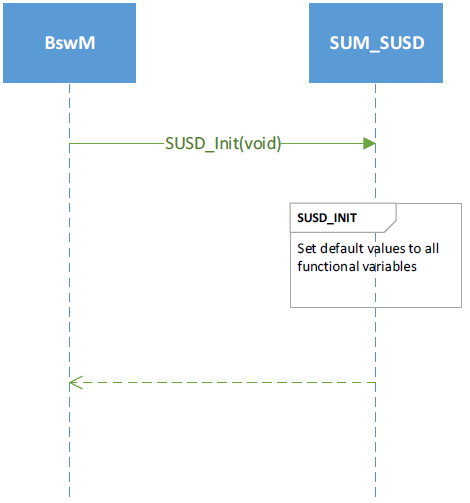
\includegraphics[width=\textwidth]{images/susd_runtime_initialization}
\end{center}
{\Satisfies{SRS_SUSD 001}}

\subsection{Wakeup Detection}
SUM_SUSD shall store all wakeup reasons in the ECU Wakeup Detection Records.

\Requirement{160}
{Wakeup records shall be initialized to 0 for a new ECU.}
{\Satisfies{SRS_SUSD 270}}

\Requirement{161}
{SUM_SUSD assumes ECU will store the wakeup reason records in non-volatile memory such that loss of battery power to the ECU does not alter the wakeup reason records. This means that the user shall configure a NvM Block Descriptor for the Wakeup Detection Records.}
{\Satisfies{SRS_SUSD 271} \Satisfies{SRS_SUSD 059}}

\Requirement{162}
{SUM_SUSD shall store the wakeup reason records chronologically, in ascending order with Data Record 1 containing the most recently stored record. Records shall be populated sequentially.}
{\Satisfies{SRS_SUSD 272} \Satisfies{SRS_SUSD 273}}

\Requirement{163}
{SUM_SUSD shall ensure that When the maximum allowable number of wakeup reason records have been stored in the PDS and the storing criteria are again met, the PDS overflows and the oldest wakeup reason record shall be deleted to allow for storage of the new wakeup reason record.}
{\Satisfies{SRS_SUSD 274}}

\Requirement{164}
{SUM_SUSD shall ensure that each record shall contain a timestamp associated to the capture of that specific record. The timestamp shall use the same value as the total vehicle operation time maintained in DID 0xF129.}
{\Satisfies{SRS_SUSD 275} \Satisfies{SRS_SUSD 059}}

\Requirement{165}
{All unknown data values and all unused bits and bytes shall be set to 0.}
{\Satisfies{SRS_SUSD 276}}

\subsection{Permit Execution}

\Requirement{147}
{\begin{center}
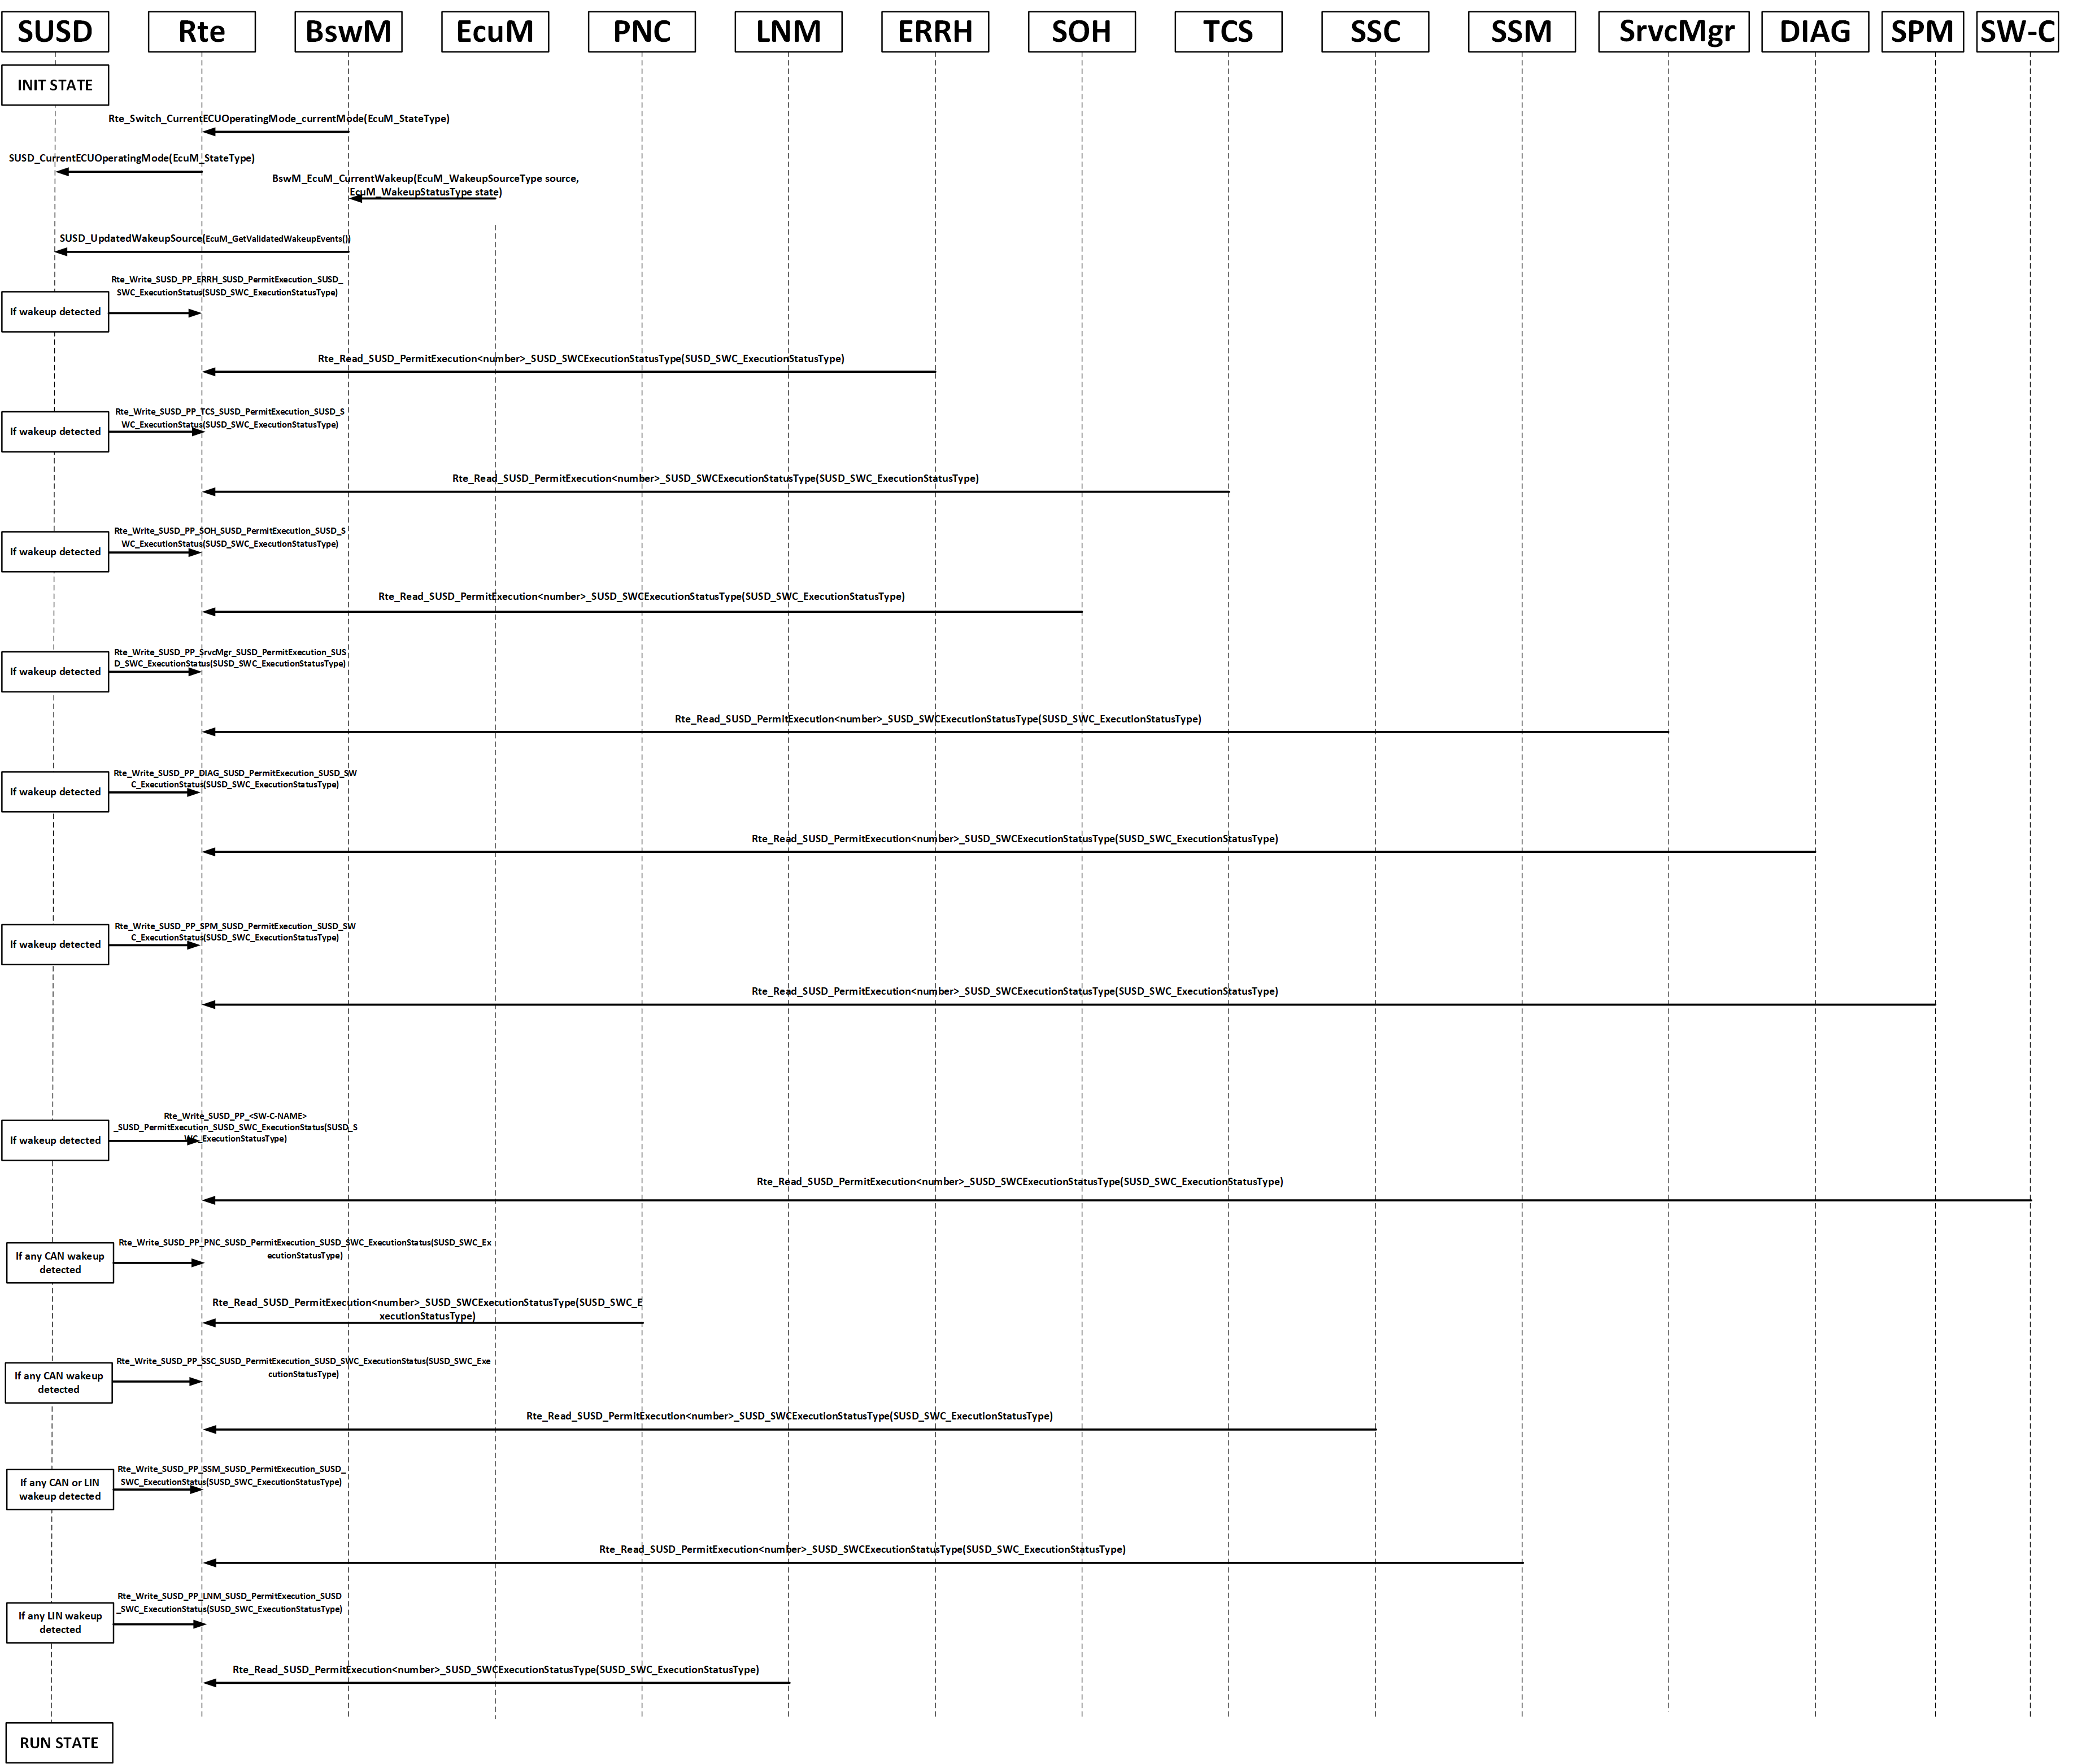
\includegraphics[width=\textwidth]{images/susd_runtime_permitexecution2}
\label{fig:susd_runtime}
\end{center}}
{\Satisfies{SRS_SUSD 004}}

\subsection{Shutdown Permission}
\label{subsec:shutdown_permission}

\Requirement{148}
{When shutdown permission signal is received from a module, SUM_SUSD updates shutdown refresh timer to \ConfigurationParameterRef{SUSD_t_Shutdown_Refresh} value for that module. If the timer expires, SUM_SUSD overrides SUM/SWC response and forces shutdown permission status to \code{Enable Shutdown} for that module.}
{\Satisfies{SRS_SUSD 019}}

\begin{center}
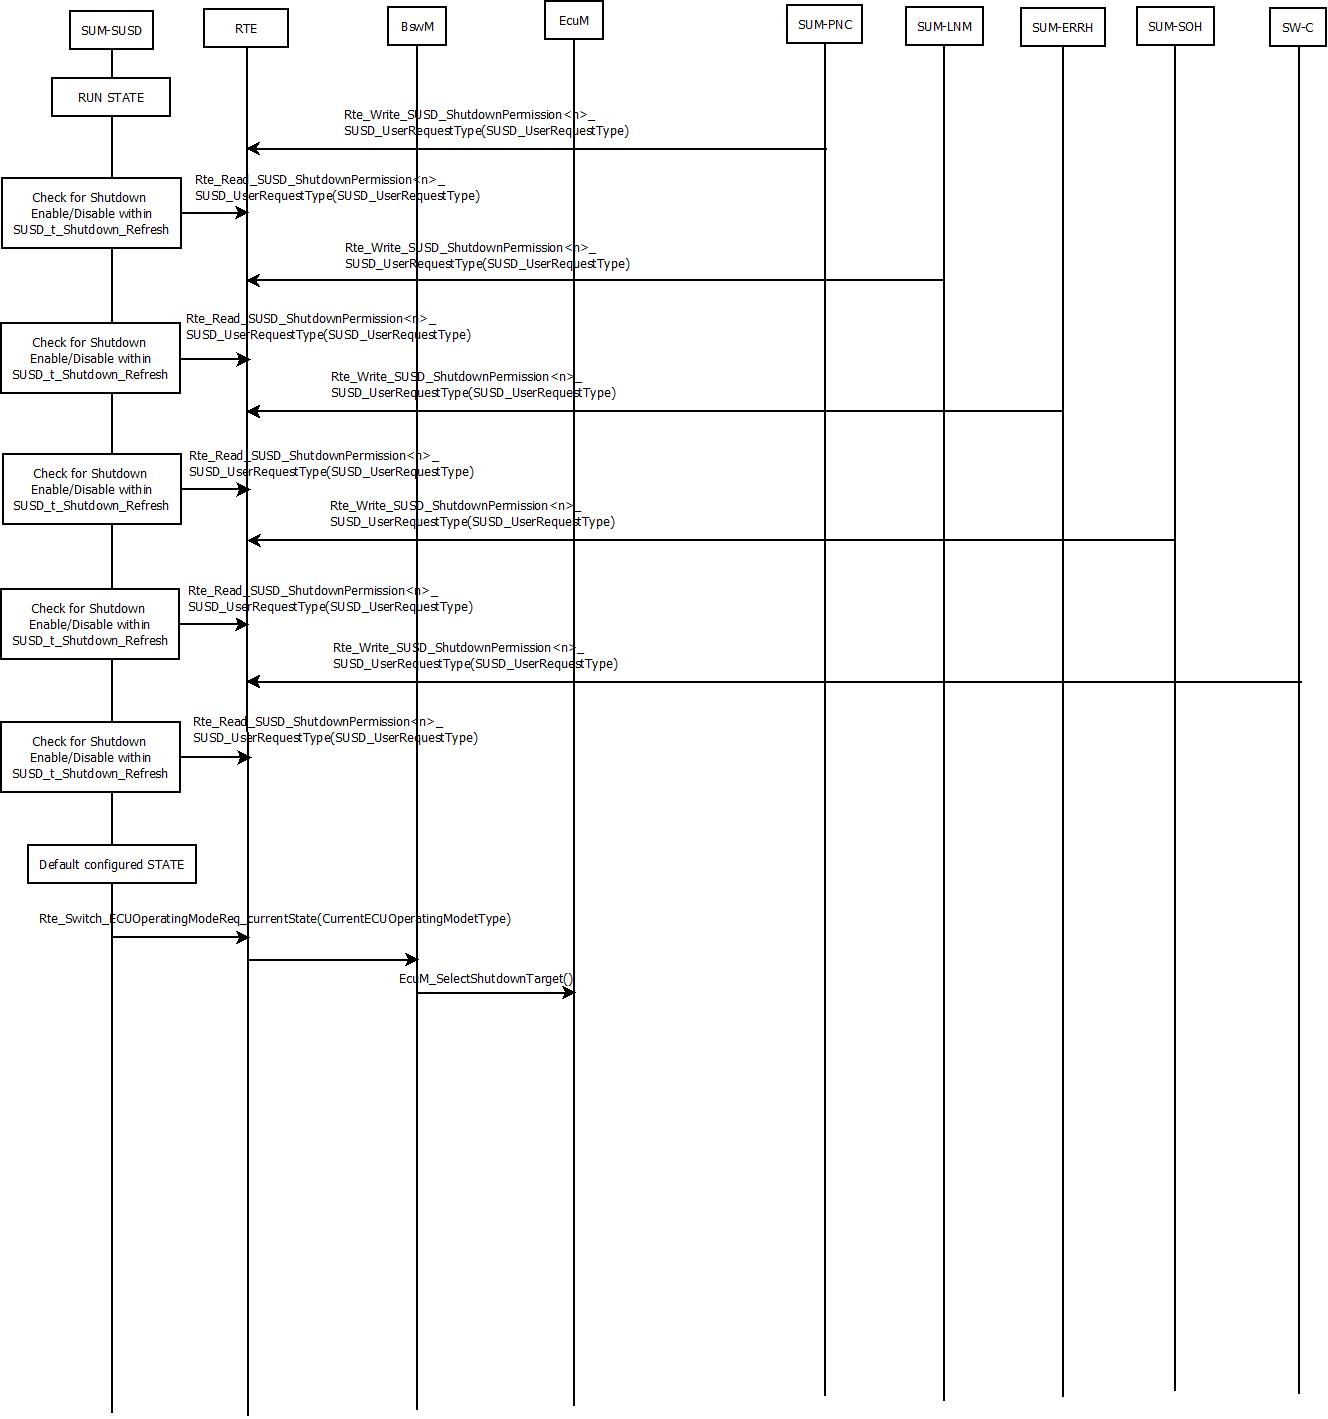
\includegraphics[width=\textwidth]{images/susd_runtime_shutdownpermission}
\end{center}

\subsection{Diagnostic Reprogramming}
\Requirement{146}
{\begin{center}
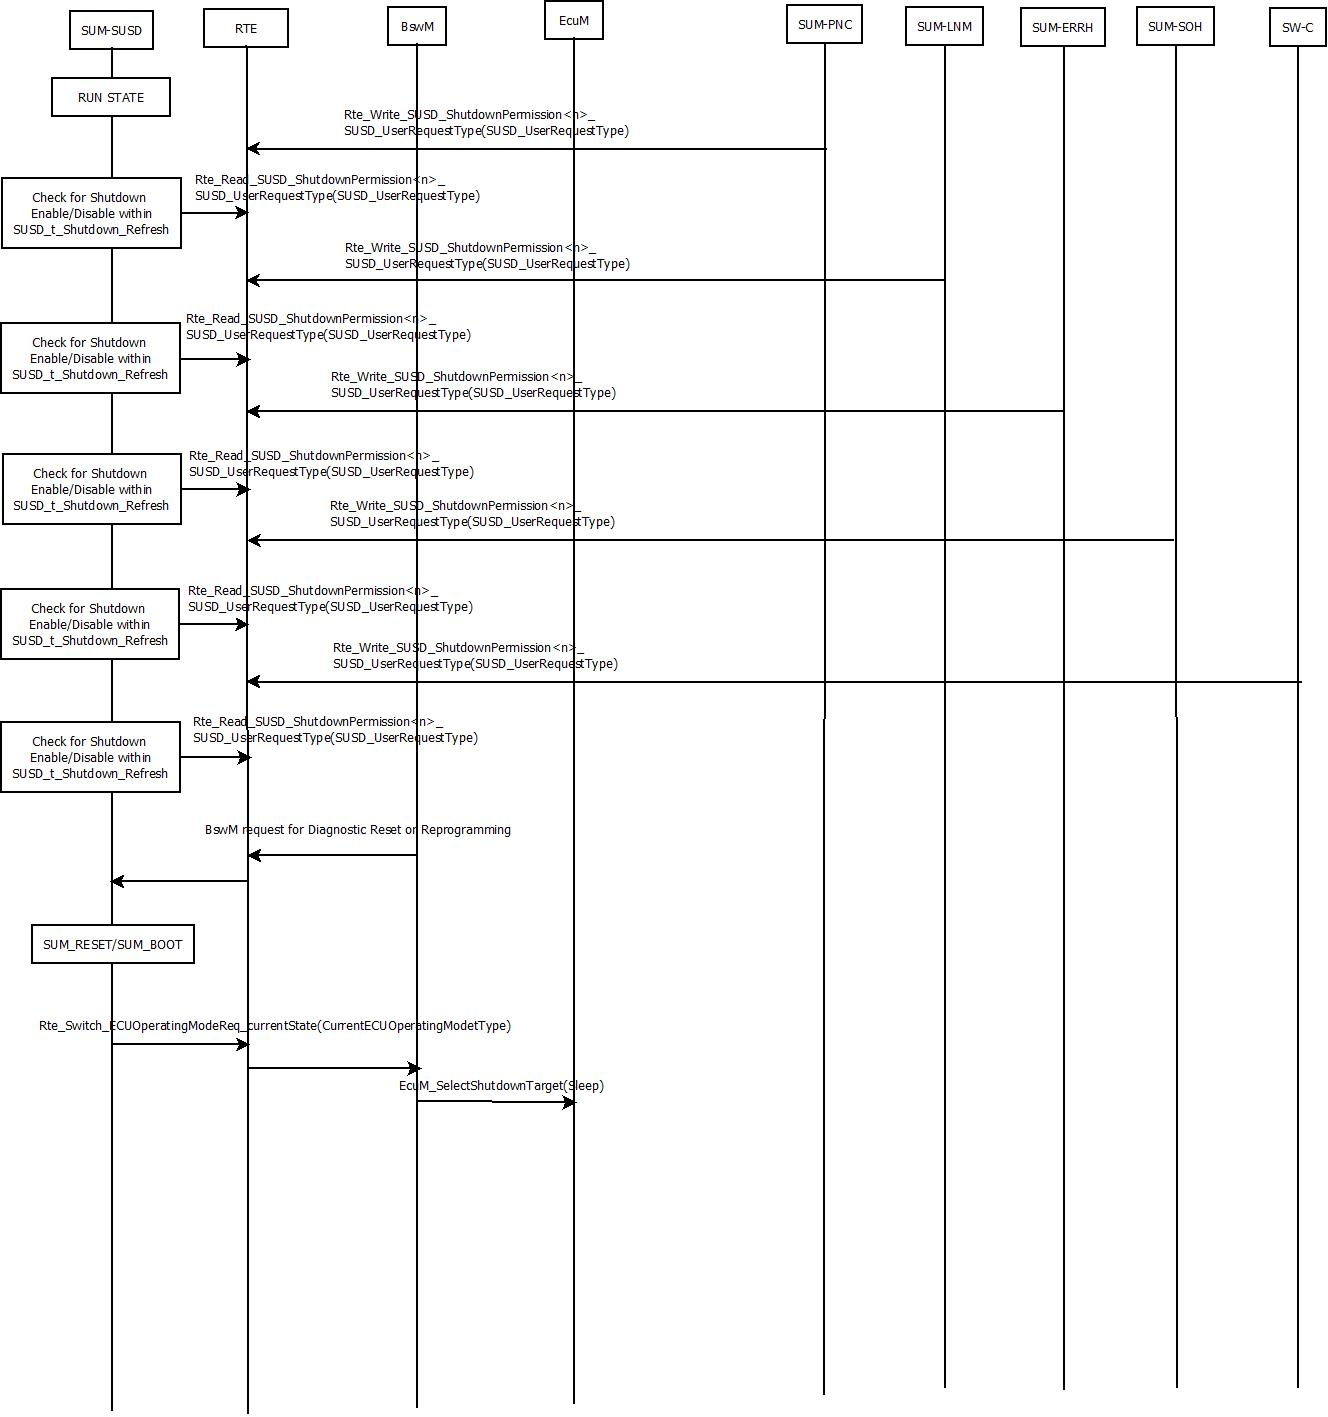
\includegraphics[width=\textwidth]{images/susd_runtime_diagnosticreprogramming}
\end{center}}
{\Satisfies{SRS_SUSD 013} \Satisfies{SRS_SUSD 022}}


\subsection{Vehicle Power Mode}
\label{sec:vehicle_power_mode}
\Requirement{149}
{Vehicle Power Mode is calculated based on availability of System Power Mode, Backup System Power mode (Power Mode Backup Strategy 1) and Run Crank (Power Mode Backup Strategy 2).
There is a calibration parameter wait time \CalibrationParameterRef{SUSD_C_RunningResetWaitTime} to receive serial data from the System Power Mode or Backup System Power Mode (Power Mode Backup Strategy 1).
\begin{itemize}
	\item After a running reset occurs, the internal timer will start and continue until it reaches the wait time defined by \CalibrationParameterRef{SUSD_C_RunningResetWaitTime}.
	\item Whenever valid data arrives from the System Power Mode or Backup System Power Mode (Power Mode Backup Strategy 1), the Vehicle Power Mode is set according to the received data, and the Fail-Soft action is not followed.
    \item If the state of the System Power Mode, Backup System Power Mode (Power Mode Backup Strategy 1), or both is UNAVAILABLE, the Fail-Soft action based on Run Crank is followed without waiting for the timer to expire.
    \item If the timer expires, the Fail-Soft action based on Run Crank is followed.
\end{itemize}
The determination of VPM varies based on safety level (QM, ASIL A) and security level (with cybersecurity risk, without cybersecurity risk).
}
{\Satisfies{SRS_SUSD 072} \Satisfies{SRS_SUSD 130} \Satisfies{SRS_SUSD 295} \Satisfies{SRS_SUSD 296} \Satisfies{SRS_SUSD 297} \Satisfies{SRS_SUSD 298} \Satisfies{SRS_SUSD 299} \Satisfies{SRS_SUSD 301}}

\Requirement{132}
{Vehicle Power Mode may assume one of the following enumerated values:
\begin{description}
\item[0x00]: OFF
\item[0x01]: ACCESSORY
\item[0x02]: RUN
\item[0x03]: START
\item[0x04]: PROPULSION
\end{description}
}
{\Satisfies{SRS_SUSD 122} \Satisfies{SRS_SUSD 142} \Satisfies{SRS_SUSD 156} \Satisfies{SRS_SUSD 173} \Satisfies{SRS_SUSD 106} \Satisfies{SRS_SUSD 183} \Satisfies{SRS_SUSD 218} \Satisfies{SRS_SUSD 253} \Satisfies{SRS_SUSD 295} \Satisfies{SRS_SUSD 296} \Satisfies{SRS_SUSD 297} \Satisfies{SRS_SUSD 298} \Satisfies{SRS_SUSD 299} \Satisfies{SRS_SUSD 301}}

\Requirement{106}
{Determination of Vehicle Power Mode at QM level without cybersecurity risk
\input{generated/tables/vpm_qm.tex}}
{\Satisfies{SRS_SUSD 130} \Satisfies{SRS_SUSD 131} \Satisfies{SRS_SUSD 137} \Satisfies{SRS_SUSD 138} \Satisfies{SRS_SUSD 139} \Satisfies{SRS_SUSD 140} \Satisfies{SRS_SUSD 141} \Satisfies{SRS_SUSD 135} \Satisfies{SRS_SUSD 136}}


\Requirement{107}
{Determination of Vehicle Power Mode at QM level with cybersecurity risk
\input{generated/tables/vpm_qm_cybersecurity.tex}}
{\Satisfies{SRS_SUSD 130} \Satisfies{SRS_SUSD 132} \Satisfies{SRS_SUSD 135} \Satisfies{SRS_SUSD 136}}

\Requirement{108}
{Determination of Vehicle Power Mode at ASIL A level without cybersecurity risk
\input{generated/tables/vpm_asil_a.tex}}
{\Satisfies{SRS_SUSD 130} \Satisfies{SRS_SUSD 133} \Satisfies{SRS_SUSD 135} \Satisfies{SRS_SUSD 136}}

\Requirement{109}
{Determination of Vehicle Power Mode at ASIL A level with cybersecurity risk
\input{generated/tables/vpm_asil_a_cybersecurity.tex}}
{\Satisfies{SRS_SUSD 130} \Satisfies{SRS_SUSD 134} \Satisfies{SRS_SUSD 135} \Satisfies{SRS_SUSD 136}}

\Requirement{175}
{Determination of Vehicle Power Mode at QM level with OBD
\input{generated/tables/vpm_qm_obd.tex}}
{\Satisfies{SRS_SUSD 130} \Satisfies{SRS_SUSD 300}}

\Requirement{110}
{SUSD shall set Vehicle Power mode state to SUM_PMS_OFF upon wakeup until Vehicle Power Mode is deterministic.}
{\Satisfies{SRS_SUSD 128}}

\Requirement{111}
{SUSD shall use last known Vehicle Power mode state upon ECU running reset.}
{\Satisfies{SRS_SUSD 129}}

\subsection{Run / Crank Active}
\label{sec:run_crank_active}

\Requirement{112}
{SUSD determines the value of Run / Crank Active based on Run/Crank Command Active from Power Mode Master and Backup Power Mode Master, and Run/Crank Input if a HW sensor is present.}
{\Satisfies{SRS_SUSD 258} \Satisfies{SRS_SUSD 148} \Satisfies{SRS_SUSD 125}}

\Requirement{113}
{Determination of Run / Crank Active
\input{generated/tables/run_crank_active.tex}}
{\Satisfies{SRS_SUSD 154} \Satisfies{SRS_SUSD 155} \Satisfies{SRS_SUSD 123} \Satisfies{SRS_SUSD 150} \Satisfies{SRS_SUSD 151} \Satisfies{SRS_SUSD 197} \Satisfies{SRS_SUSD 198} \Satisfies{SRS_SUSD 232} \Satisfies{SRS_SUSD 233}}

\subsection{Run / Crank Input}
\label{sec:run_crank_input}
This sub function samples the analog or discrete Run / Crank Input to determine its value.
It also provides the validity of the signal based on the output of the diagnostic sub functions.

\Requirement{114}
{SUSD determines the value of Run / Crank Input based on a HW sensor, if present.}
{\Satisfies{SRS_SUSD 161} \Satisfies{SRS_SUSD 258} \Satisfies{SRS_SUSD 149} \Satisfies{SRS_SUSD 196} \Satisfies{SRS_SUSD 231}}

\Requirement{115}
{SUSD determines whether Run / Crank Input is provided via a Discrete or Analog interface by reading the \CalibrationParameterRef{SUSD_C_RunCrankInputType} calibration parameter.}
{\Satisfies{SRS_SUSD 162} \Satisfies{SRS_SUSD 149} \Satisfies{SRS_SUSD 196} \Satisfies{SRS_SUSD 161} \Satisfies{SRS_SUSD 196} \Satisfies{SRS_SUSD 231}}

\subsubsection{Discrete Run / Crank Input Determination}
\Requirement{116}
{The Run/Crank Input shall be considered Low if Run/Crank Input Discrete Active is Low for a duration of \CalibrationParameterRef{SUSD_C_RunCrankInput_DebounceTime}.

The Run/Crank Input shall be considered High if Run/Crank Input Discrete Active is High for a duration of \CalibrationParameterRef{SUSD_C_RunCrankInput_DebounceTime}.
}
{\Satisfies{SRS_SUSD 162} \Satisfies{SRS_SUSD 170} \Satisfies{SRS_SUSD 171}}

\subsubsection{Analog Run / Crank Input Determination}
\Requirement{117}
{The Run / Crank Input shall be considered Low when Run / Crank Input Voltage is less than calibration parameter \CalibrationParameterRef{SUSD_C_RunCrankInputThresholdLow} voltage for a duration of \CalibrationParameterRef{SUSD_C_RunCrankInput_DebounceTime}.

The Run / Crank Input shall be considered High when Run / Crank Input Voltage is greater than calibration \CalibrationParameterRef{SUSD_C_RunCrankInputThresholdHigh} voltage for a duration of \CalibrationParameterRef{SUSD_C_RunCrankInput_DebounceTime}.
}
{\Satisfies{SRS_SUSD 168} \Satisfies{SRS_SUSD 169}}

\subsubsection{Run / Crank Input Voltage Determination}
\Requirement{118}
{The Run/Crank Input Voltage shall be determined by converting the input signal Run/Crank Input Percentage using the \CalibrationParameterRef{SUSD_C_PerToVoltageConvFactor} calibration parameter.
}
{\Satisfies{SRS_SUSD 178} \Satisfies{SRS_SUSD 179} \Satisfies{SRS_SUSD 180} \Satisfies{SRS_SUSD 182}}

\subsubsection{Run / Crank Input Validity Determination}
\Requirement{119}
{Run / Crank Input Invalidity shall be set to TRUE if either Run/Crank Input Stuck High Diagnostic Fault Active or Run/Crank Input Stuck Low Diagnostic Fault Active are TRUE.
}
{\Satisfies{SRS_SUSD 172} \Satisfies{SRS_SUSD 163} \Satisfies{SRS_SUSD 164}}

\subsection{Run / Crank Input Stuck High / Low Diagnostic}
\label{sec:run_crank_input_stuck}

\subsubsection{Run / Crank Input Stuck High Diagnostic}

\Requirement{120}
{This sub function provides Stuck High Diagnostic for Run/Crank Input (whether discrete or analog) for a given controller.
}
{\Satisfies{SRS_SUSD 188} \Satisfies{SRS_SUSD 189} \Satisfies{SRS_SUSD 190}}

\Requirement{121}
{The Run Crank Input Stuck High diagnostic shall be enabled when all the following conditions are TRUE:
\begin{itemize}
\item The calibration parameter \CalibrationParameterRef{SUSD_C_RunCrankInputStuckHi_Enable} is TRUE.
\item The battery voltage is in the operating voltage of 9.5V and above with a hysteresis of 0.5V when it goes low.
\item The Primary Run / Crank Command State from Power Mode Master is AVAILABLE, VALID, with no FoFA and LOW,
or the The Secondary Run / Crank Command State from Backup Power Mode Master is AVAILABLE, VALID, with no FoFA and LOW
when the Primary Run / Crank Command State from Power Mode Master is UNAVAILABLE or INVALID or with FoFA.
\end{itemize}
}
{\Satisfies{SRS_SUSD 201}}

\Requirement{122}
{The Run / Crank Stuck High diagnostic failure criteria shall be met if the input signal Run / Crank Input is High.
}
{\Satisfies{SRS_SUSD 202}}

\Requirement{123}
{The Run / Crank Stuck High diagnostic shall notify SUM_ERRH of errors by using the Run / Crank Input Stuck High Diagnostic Status interface.
}
{\Satisfies{SRS_SUSD 203} \Satisfies{SRS_SUSD 204}}

\Requirement{124}
{Run / Crank Input Stuck High Diagnostic Status shall be set to Diagnostic Failed (\code{SUSD_DIAGNOSTIC_FAILED}) for one execution when the accumulated number of executions where the Enable Criteria and Failure Criteria were met is equal to or greater than the calibration parameter \CalibrationParameterRef{SUSD_C_RunCrankInputStuckHi_FailCount}.

Run / Crank Input Stuck High Diagnostic Status shall be set to Diagnostic Passed (\code{SUSD_DIAGNOSTIC_PASSED}) for one execution when all of the following are true:
\begin{itemize}
\item the accumulated number of executions where the Enable Criteria and Failure Criteria were met is less than the calibration parameter \CalibrationParameterRef{SUSD_C_RunCrankInputStuckHi_FailCount}.
\item the accumulated number of executions where the Enable Criteria were met is equal to or greater than the calibration parameter \CalibrationParameterRef{SUSD_C_RunCrankInputStuckHi_SampleCount}.
\end{itemize}

Run / Crank Input Stuck High Diagnostic Status shall be set to No Status To Report (\code{SUSD_DIAGNOSTIC_NO_STATUS_TO_REPORT}) when the Run / Crank Input Stuck High Diagnostic Status is not presently being set to Diagnostic Failed or Diagnostic Passed.

The accumulated number of executions where the Enable Criteria and Failure Criteria were met, and the accumulated number of executions where the diagnostic monitor's Enable Criteria were met, shall both be reset when any of the following are true:
\begin{itemize}
\item Run / Crank Input Stuck High Diagnostic Status is set to Diagnostic Failed
\item Run / Crank Input Stuck High Diagnostic Status is set to Diagnostic Passed
\item Upon controller initialization
\end{itemize}
}
{\Satisfies{SRS_SUSD 205} \Satisfies{SRS_SUSD 206} \Satisfies{SRS_SUSD 207} \Satisfies{SRS_SUSD 208}}

\Requirement{125}
{Run / Crank Input Stuck High Diagnostic Fault Active shall be set equal to the value of the Run / Crank Input Stuck High Diagnostic Fault Active Status Request received from SUM_ERRH.
}
{\Satisfies{SRS_SUSD 191}}

\subsubsection{Run / Crank Input Stuck Low Diagnostic}

\Requirement{126}
{This sub function provides Stuck Low Diagnostic for Run/Crank Input (whether discrete or analog) for a given controller.
}
{\Satisfies{SRS_SUSD 223} \Satisfies{SRS_SUSD 224} \Satisfies{SRS_SUSD 225}}

\Requirement{127}
{The Run Crank Input Stuck Low diagnostic shall be enabled when all the following conditions are TRUE:
\begin{itemize}
\item The calibration parameter \CalibrationParameterRef{SUSD_C_RunCrankInputStuckLow_Enable} is TRUE.
\item The battery voltage is in the operating voltage of 9.5V and above with a hysteresis of 0.5V when it goes low.
\item The Primary Run / Crank Command State from Power Mode Master is AVAILABLE, VALID, with no FoFA and HIGH,
or the The Secondary Run / Crank Command State from Backup Power Mode Master is AVAILABLE, VALID, with no FoFA and HIGH
when the Primary Run / Crank Command State from Power Mode Master is UNAVAILABLE or INVALID or with FoFA.
\end{itemize}
}
{\Satisfies{SRS_SUSD 237}}

\Requirement{128}
{The Run / Crank Stuck Low diagnostic failure criteria shall be met if the input signal Run / Crank Input is Low.
}
{\Satisfies{SRS_SUSD 260}}

\Requirement{129}
{The Run / Crank Stuck Low diagnostic shall notify SUM_ERRH of errors by using the Run / Crank Input Stuck Low Diagnostic Status interface.
}
{\Satisfies{SRS_SUSD 238} \Satisfies{SRS_SUSD 239}}

\Requirement{130}
{Run / Crank Input Stuck Low Diagnostic Status shall be set to Diagnostic Failed (\code{SUSD_DIAGNOSTIC_FAILED}) for one execution when the accumulated number of executions where the Enable Criteria and Failure Criteria were met is equal to or greater than the calibration parameter \CalibrationParameterRef{SUSD_C_RunCrankInputStuckLow_FailCount}.

Run / Crank Input Stuck Low Diagnostic Status shall be set to Diagnostic Passed (\code{SUSD_DIAGNOSTIC_PASSED}) for one execution when all of the following are true:
\begin{itemize}
\item the accumulated number of executions where the Enable Criteria and Failure Criteria were met is less than the calibration parameter \CalibrationParameterRef{SUSD_C_RunCrankInputStuckLow_FailCount}.
\item the accumulated number of executions where the Enable Criteria were met is equal to or greater than the calibration parameter \CalibrationParameterRef{SUSD_C_RunCrankInputStuckLow_SampleCount}.
\end{itemize}

Run / Crank Input Stuck Low Diagnostic Status shall be set to No Status To Report (\code{SUSD_DIAGNOSTIC_NO_STATUS_TO_REPORT}) when the Run / Crank Input Stuck Low Diagnostic Status is not presently being set to Diagnostic Failed or Diagnostic Passed.

The accumulated number of executions where the Enable Criteria and Failure Criteria were met, and the accumulated number of executions where the diagnostic monitor's Enable Criteria were met, shall both be reset when any of the following are true:
\begin{itemize}
\item Run / Crank Input Stuck Low Diagnostic Status is set to Diagnostic Failed
\item Run / Crank Input Stuck Low Diagnostic Status is set to Diagnostic Passed
\item Upon controller initialization
\end{itemize}
}
{\Satisfies{SRS_SUSD 240} \Satisfies{SRS_SUSD 241} \Satisfies{SRS_SUSD 242} \Satisfies{SRS_SUSD 243} \Satisfies{SRS_SUSD 226}}

\Requirement{131}
{Run / Crank Input Stuck Low Diagnostic Fault Active shall be set equal to the value of the Run / Crank Input Stuck Low Diagnostic Fault Active Status Request received from SUM_ERRH.
}
{\Satisfies{SRS_SUSD 252}}

\subsection{Battery Voltage}\label{subsec:battery_voltage}

\Requirement{138}
{Input – VehicleBatteryVoltage which shall be provided as BatteryVoltage_Actual.

The received voltage is checked against the calibration parameters \ConfigurationParameterRef{SUSD_C_UnderVoltage_hysteresis} and \ConfigurationParameterRef{SUSD_C_OverVoltage_hysteresis} to provide the \code{BatteryVoltageRange<Min V>To<Max V>} to SW-C on normal, under and over voltage operating range. \newline

For each configured SUSD_C_BatteryVoltageRange, a corresponding port PP_SUSD_BatteryVoltage_MintoMax_<RangeName> is generated. \newline

There is always one default voltage range is 9V-16V and go with the calibration parameters \ConfigurationParameterRef{SUSD_C_UnderVoltage_hysteresis} and \ConfigurationParameterRef{SUSD_C_OverVoltage_hysteresis} to provide the voltage operating range.
Port PP_SUSD_DefaultBatteryVoltage_MintoMax_9Vto16V is always generated, it is used with 9V-16V default range. \newline

If a SUSD_C_SWCInfo does not refer to any voltage range, it implicitly goes with 9V-16V default range and is notified about voltage level by PP_SUSD_DefaultBatteryVoltage_MintoMax_9Vto16V port. \newline

The received voltage is checked against the calibration parameter \CalibrationParameterRef{SUSD_C_DisableNVMWrite_Voltage} to know when to set the \code{BattVoltage_DisableNVMWrite} interface.}
{\Satisfies{SRS_SUSD 240} \Satisfies{SRS_SUSD 104} \Satisfies{SRS_SUSD 030} \Satisfies{SRS_SUSD 153} \Satisfies{SRS_SUSD 105} \Satisfies{SRS_SUSD 110}}

\Requirement{246}
{SUM\_SUSD shall read the battery voltage sensor status from the supplier SWC via the \code{BattVltgSnsrStsAvl} port interface. The received \code{BattVltgSnsrStsEnum} signal indicates the availability of the battery voltage reading: value 1 means Battery\_Voltage\_Not\_Available, value 2 means Battery\_Voltage\_Available.}
{\Satisfies{SRS_SUSD 332}}

\Requirement{247}
{SUM\_SUSD shall enable NVM write (set \code{BattVoltage\_DisableNVMWrite} to 0) only when BOTH the vehicle battery voltage is greater than or equal to the calibration parameter \CalibrationParameterRef{SUSD_C_DisableNVMWrite_Voltage} AND the battery voltage sensor status is \code{Battery\_Voltage\_Available} (BattVltgSnsrStsEnum == 2). In all other cases, SUM\_SUSD shall disable NVM write (set \code{BattVoltage\_DisableNVMWrite} to 1) to avoid NVM corruption during low voltage transients or when the voltage sensor is not available.}
{\Satisfies{SRS_SUSD 333}}

\subsection{Battery State of Charge}
\Requirement{167}
{If the configuration parameter SUSD\_Battery\_State\_of\_Charge\_Supported is set to true, SUM\_SUSD checks the vehicle battery state of charge whenever the Runnable RE\_SUSD\_BatteryNotifications is invoked.
This functionality is implemented by reading the interface VehicleBatteryStateOfCharge. 

SUM\_SUSD notifies the BswM through the BatteryCharge_DisableWkups interface independently of the fact that the value, read from the interface VehicleBatteryStateOfCharge, is equal to '0' (low charge) or '1' (normal charge).
In particular, when the state of charge is low, SUM\_SUSD updates the BatteryCharge_DisableWkups interface by writing '1'. Otherwise, if the state of charge is normal, SUM\_SUSD updates the interface by writing '0'.}
{\Satisfies{SRS_SUSD 033}}

\subsection{Wakeup detection}\label{sec:wake_updetection}
\Requirement{166}
{If no wakeup is active, SUM\_SUSD resets the wakeup bits in the SUSD\_<SUM/SWC>\_PermitExecution interfaces, otherwise, if at least one wakeup is active SUM\_SUSD
sets the wakeup bits in the PermitExecution interfaces of SUM\_ERRH, SUM\_TCS, SUM\_SOH, SUM\_SrvcMgr, SUM\_DIAG and SUM\_SPM. Moreover, in this case, it also sets the wakeup bit in the 
PermitExecution interface of each SW-C. 

If no CAN-related wakeup is active, SUM\_SUSD resets the wakeup bit in the PermitExecution interfaces of SUM\_SSC and SUM\_PNC, 
otherwise, if at least a CAN-related wakeup is active, SUM\_SUSD sets the wakeup bit in the PermitExecution interfaces of SUM\_SSC and SUM\_PNC. Similarly,  
if no LIN-related wakeup is active, SUM\_SUSD resets the wakeup bit in the PermitExecution interfaces of SUM\_LNM, 
otherwise, if at least a LIN-related wakeup is active, SUM\_SUSD sets it. 

Finally, if no CAN-related or LIN-related wakeup is active, SUM\_SUSD resets the wakeup bit 
in the PermitExecution interface of SUM\_SSM, otherwise, if at least a CAN-related wakeup or a LIN-related wakeup is active, SUM\_SUSD sets the bit.

SUM\_SUSD also maintains a list of the active ECU wakeups and resets this list during the initialization.}
{\Satisfies{SRS_SUSD 044} \Satisfies{SRS_SUSD 045}\Satisfies{SRS_SUSD 046}}\newline
{\Satisfies{SRS_SUSD 047} \Satisfies{SRS_SUSD 049} \Satisfies{SRS_SUSD 051}}\newline 

\subsection{Reset and Shutdown Target bits management}\label{sec:reset_shutdown_target}
\Requirement{168}
{When a diagnostic reset  or a reprogramming request occurs, SUM\_SUSD resets the Reset bit in the SUM/SW-C PermitExecution interfaces.
Moreover, in case of a diagnostic reset, SUM\_SUSD also sets the Shutdown Target bit in the SUM/SW-C PermitExecution interfaces.}
{\Satisfies{SRS_SUSD 280} \Satisfies{SRS_SUSD 281}\Satisfies{SRS_SUSD 098}}

\subsection{Determination of the type of reset}\label{sec:reset_shutdown_target}
\Requirement{169}

{The SUM_SUSD determines if an ECU did undergo a reset as well as the type of reset. In particular, when a diagnostic reset request occurs, the SUM_SUSD resets the Reset bit in the
SUM/SW-C PermitExecution interfaces and starts the SUM\_SUSD\_RESETExecution\_TIMER. This is a 2-byte unsigned integer variable that is initialized to zero immediately after that
the first wake-up occurs. 

When it is started, the SUM\_SUSD\_RESETExecution\_TIMER is incremented by one every millisecond until the system is ready to reset. When this happens,
 the last value of the timer is stored into NvM and, then, the SUM\_SUSD asks the BSW to reset the ECU.
 Once the SUM\_SUSD\_RESETExecution\_TIMER has been started, the SUM\_SUSD shall not request a normal shutdown (SUM\_SLEEP) for the remainder of the diagnostic reset sequence.

 At reset, the ECU will be woken up by a well-defined wake-up source. The SUM\_SUSD identifies the wake-up source by interfacing with the BSW and detects the type of reset by
 reading the value of the SUM\_SUSD\_RESETExecution\_TIMER stored into NvM. In particular, if the wake-up source is ECUM\_WKSOURCE\_RESET or ECUM\_WKSOURCE\_INTERNAL\_RESET 
 or ECUM\_WKSOURCE\_INTERNAL\_WDG or ECUM\_WKSOURCE\_EXTERNAL\_WDG:
\begin{enumerate}
\item if SUM\_SUSD\_RESETExecution\_TIMER $>$ SUM\_SUSD\_RESETExecution\_TIMER\_Thresh, the SUM\_SUSD notifies the SUM\_SOH that a delayed Reset occurred by setting 
the SUSD\_SOH\_ResetOccured interface to $0\text{x}1$.
\item otherwise, if SUM\_SUSD\_RESETExecution\_TIMER $\le$ SUM\_SUSD\_RESETExecution\_TIMER\_Thresh, the SUM\_SUSD notifies the SUM\_SOH that an immediate Reset occurred
 by setting the SUSD\_SOH\_ResetOccured interface to $0\text{x}2$.
\end{enumerate}
}
{\Satisfies{SRS_SUSD 282} \Satisfies{SRS_SUSD 283} \Satisfies{SRS_SUSD 285} \Satisfies{SRS_SUSD 286} \Satisfies{SRS_SUSD 288} \Satisfies{SRS_SUSD 289} \Satisfies{SRS_SUSD 291} \Satisfies{SRS_SUSD 292} \Satisfies{SRS_SUSD 293} \Satisfies{SRS_SUSD 294}}



\subsection{Activity Records}\label{sec:activity_records}

\Requirement{177}
{SUM_SUSD is responsible for implementing the DID 0xE0D7 and RID 0x041A to monitor and report the activity records.}
{\Satisfies{SRS_SUSD 306} \Satisfies{SRS_SUSD 320} \Satisfies{SRS_SUSD 324}}

\Requirement{178}
{SUM_SUSD keeps track of the following information to fulfill the DID 0xE0D7 requirements:
\begin{itemize}
	\item Total Activity Timer
	\item Total Wakeup Counter
	\item Active Delay Timer
	\item Monitor Disabled
	\item Activity Records; including:
	\begin{itemize}
		\item Record ID
		\item Record Wakeup Reason
		\item Record Last Active Reason
		\item Record Current Activity Timer
		\item Record Total Activity Timer
		\item Record Wakeup Counter
		\item Record Position in DID (to be used internally - not included in DID)
	\end{itemize}
	\item Next Available Position in DID (to be used internally - not included in DID)
\end{itemize}
}
{\Satisfies{SRS_SUSD 306}}

\Requirement{179}
{\code{RE_Sum_SUSD_ActivityRecord_Handler} is responsible for handling the state machine of activity records and will be called by the periodicity defined using \code{Sum_SUSD_AR_Periodicity}.}
{\Satisfies{SRS_SUSD 306}}

\Requirement{214}
{\code{RE_Sum_SUSD_ActivityRecord_Handler} shall monitor the ECU Voltage through \code{RP_SUSD_VehicleBatteryVoltage_VehicleVoltage}.}
{\Satisfies{SRS_SUSD 309}}

\Requirement{189}
{In \code{RE_Sum_SUSD_ActivityRecord_Handler}, a timer called \code{Sum_SUSD_AR_VoltageOver12_Timer} will be incremented by the periodicity of \code{Sum_SUSD_AR_Periodicity} if the voltage is over 12V.}
{\Satisfies{SRS_SUSD 310}}

\Requirement{190}
{The \code{Sum_SUSD_AR_VoltageOver12_Timer} shall reset to zero if the voltage is equal or less than 12V.}
{\Satisfies{SRS_SUSD 310}}

\Requirement{191}
{In \code{RE_Sum_SUSD_ActivityRecord_Handler}, a timer called \code{Sum_SUSD_AR_Propulsion_Timer} will be incremented by the periodicity of \code{Sum_SUSD_AR_Periodicity} if the \code{Vehicle Power Mode} is equal to Propulsion.}
{\Satisfies{SRS_SUSD 310}}

\Requirement{192}
{The \code{Sum_SUSD_AR_Propulsion_Timer} shall reset to zero if the \code{Vehicle Power Mode} is no longer equal to Propulsion.}
{\Satisfies{SRS_SUSD 310}}

\Requirement{215}
{In \code{RE_Sum_SUSD_ActivityRecord_Handler}, a timer called \code{Sum_SUSD_AR_VoltageUnder10_Timer} will be incremented by the periodicity of \code{Sum_SUSD_AR_Periodicity} if the voltage is less than 10V.}
{\Satisfies{SRS_SUSD 309}}

\Requirement{216}
{The \code{Sum_SUSD_AR_VoltageUnder10_Timer} shall reset to zero if the voltage is equal or greater than 10V.}
{\Satisfies{SRS_SUSD 309}}


\Requirement{242}
{
\textbf{SPM and SUSD Synchronization} \\
The \code{SPM_SUSD_ActivityRecordCmd} interface will synchronize communication between SPM and SUSD.

SUSD shall inform SPM of any of the following events:
\begin{itemize}
    \item NvM writes needed,
    \item any clearing of the content needed,
    \item the start of a record update,
    \item the stop of a record update.
\end{itemize}
This ensures that SPM can correctly trigger the recovery of DIDs and maintain synchronization with SUSD.
}
{\Satisfies{SRS_SUSD 328} \Satisfies{SRS_SUSD 329}}

\subsubsection{WakeUp/Initialization State}

\Requirement{180}
{\code{Sum_SUSD_ActivityRecord_WakeUp_Handler} is responsible for handling the state machine of activity records. 
The \code{Sum_SUSD_ActivityRecord_WakeUp_Handler} is called by \code{Sum_SUSD_ActivityRecord_Handler} whenever the current state is \code{Sum_SUSD_AR_State_Wakeup}.}
{\Satisfies{SRS_SUSD 307}}

\Requirement{181}
{Upon the first initialization after the flash the \code{Sum_SUSD_ActivityRecord_Clear()} will be called to reset the following:
\begin{itemize}
	\item Total Activity Timer
	\item Total Wakeup Counter
	\item Activity Records
\end{itemize}
Furthermore, Active Delay Timer will be reset and Monitor Disabled set to FALSE.
}
{\Satisfies{SRS_SUSD 307} \Satisfies{SRS_SUSD 314} \Satisfies{SRS_SUSD 318}}

\Requirement{182}
{In order to understand if the boot is the first boot after the flash, the flag \code{Sum_SUSD_FirstBootAfterFlash} shall be stored on NvM and checked at the time of boot. 
If the flag on NvM is not set, it means that the current wakeup is the first one after the flash. The SUM_SUSD, then, sets the flag and stores it on NvM.}
{\Satisfies{SRS_SUSD 307}}

\Requirement{183}
{Upon further initialization (from the 2nd one after flash), if the \code{Monitor Disabled} is set to True for any reason, the Activity Record state machine moves to Disabled state.}
{\Satisfies{SRS_SUSD 307}}

\Requirement{184}
{Otherwise, if the \code{Monitor Disabled} is set to False, the \code{Total Wakeup Counter} shall be incremented. Then the next step is determined by \code{Vehicle Power Mode}.}
{\Satisfies{SRS_SUSD 307}}

\Requirement{185}
{If the Vehicle Power Mode stored in \code{SUSD_VehiclePowerMode} is equal to Propulsion, the next state will be Inactive state.}
{\Satisfies{SRS_SUSD 307}}

\Requirement{186}
{If the Vehicle Power Mode stored in \code{SUSD_VehiclePowerMode} is not equal to Propulsion, the next state will be an intermediatory state \code{Sum_SUSD_AR_State_ToActive} to check the conditions prior to moving to Active state.}
{\Satisfies{SRS_SUSD 307}}



\subsubsection{Disabled State}

\Requirement{187}
{\code{Sum_SUSD_ActivityRecord_Disabled_Handler} is responsible for handling the state machine of activity records during Disabled state. 
The \code{Sum_SUSD_ActivityRecord_Disabled_Handler} is called by \code{Sum_SUSD_ActivityRecord_Handler} whenever the current state is \code{Sum_SUSD_AR_State_Disabled}.}
{\Satisfies{SRS_SUSD 310}}

\Requirement{193}
{In this state, if the \code{Sum_SUSD_AR_Propulsion_Timer} is greater or equal to 60 seconds and the \code{Sum_SUSD_AR_VoltageOver12_Timer} is greater or equal to 10 seconds at the same time,
the \code{Monitor Disabled} shall set to False and the state machine shall move to \code{Inactive} state.}
{\Satisfies{SRS_SUSD 310} \Satisfies{SRS_SUSD 314}}



\subsubsection{Inactive State}
\label{subsec:inactive_state}
\Requirement{195}
{\code{Sum_SUSD_ActivityRecord_Inactive_Handler} is responsible for handling the state machine of activity records during Inactive state. 
The \code{Sum_SUSD_ActivityRecord_Inactive_Handler} is called by \code{Sum_SUSD_ActivityRecord_Handler} whenever the current state is \code{Sum_SUSD_AR_State_Inactive} and \code{Monitor Disabled} is set to \code{FALSE}.}
{\Satisfies{SRS_SUSD 308}}

\Requirement{196}
{During this state, while the \code{Vehicle Power Mode} is not equal to Propulsion, the Activity Delay Timer called \code{Sum_SUSD_AR_ActiveDelay_Timer} will be incremented by the periodicity \code{SUSD_AR_PERIODICITY}.}
{\Satisfies{SRS_SUSD 308} \Satisfies{SRS_SUSD 315} \Satisfies{SRS_SUSD 316}}

\Requirement{197}
{During this state, while the \code{Vehicle Power Mode} is not equal to Propulsion, if \code{Sum_SUSD_AR_ActiveDelay_Timer} exceeds the \code{k_AR_Active_Delay} calibration parameter or if \code{SUSD_GaaSUMShutdownPermission} associated to PNCs is equal to \code{ENABLESHUTDOWN} (exiting COMM_ACTIVE which means all PNCs are FALSE), the following parameters shall be reset:
\begin{itemize}
	\item Activity Records
	\item Total Activity Timer
	\item Total WakeUp Counter
\end{itemize}
Only once the \code{Sum_SUSD_AR_ActiveDelay_Timer} exceeds the \code{k_AR_Active_Delay} calibration parameter, the state machine shall move to Active state directly.
}
{\Satisfies{SRS_SUSD 308} \Satisfies{SRS_SUSD 313}}

\Requirement{198}
{During this state, whenever the \code{Vehicle Power Mode} is set to Propulsion, the \code{Sum_SUSD_AR_ActiveDelay_Timer} will be reset to zero.}
{\Satisfies{SRS_SUSD 308}}



\subsubsection{Initialization to Active Check State}

\Requirement{199}
{\code{Sum_SUSD_ActivityRecord_ToActive_Handler} is responsible for handling the state machine of activity records when the state is moving from \code{Sum_SUSD_AR_State_Wakeup} to \code{Sum_SUSD_AR_State_Active}. 
The \code{Sum_SUSD_ActivityRecord_ToActive_Handler} is called by \code{Sum_SUSD_ActivityRecord_Handler} whenever the current state is \code{Sum_SUSD_AR_State_ToActive}.}
{\Satisfies{SRS_SUSD 306}}

\Requirement{200}
{The last wake up source and reason is recorded on RAM through the \code{Sum_SUSD_ActivityRecordUpdated}. The wakeup source can be determined by internal Record_\{X\}_Counter and the reason can be determined by internal reason active array or bit-map. (Refer to ~\ref{subsec:update_record})}
{\Satisfies{SRS_SUSD 322} \Satisfies{SRS_SUSD 323} \Satisfies{SRS_SUSD 325}}

\Requirement{201}
{Whenever the wake up source is Record 0x02 or 0x03 \code{Record \{X\}}, the following steps shall be executed:
\begin{enumerate}
	\item The state machine of Activity Record shall move to \code{Sum_SUSD_AR_State_Active} state.
	\item If the \code{Record \{X\} Position in DID} is equal to \code{0xFF} (not inserted), the \code{Record \{X\} Position in DID} shall be updated by the \code{Next Available Position in DID} and the later should be incremented. Moreover, the \code{Reason ID} on that position shall be updated.
	\item Using the RAM copy of DID and the currently known position of \code{Record \{X\}}, the \code{Record \{X\} Wake Up Counter} shall be incremented.
	\item Using the RAM copy of DID and the currently known position of \code{Record \{X\}}, the \code{Record \{X\} Last Wake Up Reason} shall be populated. 
\end{enumerate}
}
{\Satisfies{SRS_SUSD 306}}

\Requirement{202}
{A timer called \code{Sum_SUSD_AR_InitDelay_Timer} shall be started and incremented by the periodicity of \code{Sum_SUSD_AR_Periodicity}.}
{\Satisfies{SRS_SUSD 306}}

\Requirement{203}
{If a wake up with reason 0x20 to 0x25 is called before \code{Sum_SUSD_AR_InitDelay_Timer} passes (be greater than) \code{k_AR_Init_Delay}, the reason is determined through the received wake up reason.
Otherwise, if a wake up with reason 0x26 is detected during the init delay period, \code{Sum_SUSD_Match_0x26_WakeupSource} shall be invoked to evaluate the wakeup source. This function may:
\begin{itemize}
\item Reset \code{Sum_SUSD_AR_InitDelay_Timer} and update the waiting flag \code{waiting_on_local_PN_AP_WUF_activations} accordingly based on the detected wakeup condition, or
\item Handle the wakeup source transition to Active state if applicable.
\end{itemize}
If no local PN/AP/WUF activation occurs before \code{Sum_SUSD_AR_InitDelay_Timer} exceeds \code{k_AR_Init_Delay}, the timer shall be stopped and the reason is assumed to be 0x01. Then:
\begin{enumerate}
\item The state machine of Activity Record shall move to \code{Sum_SUSD_AR_State_Active} state.
\item If the \code{Record \{X\} Position in DID} is equal to \code{0xFF} (not inserted), the \code{Record \{X\} Position in DID} shall be updated by the \code{Next Available Position in DID} and the later should be incremented. Moreover, the \code{Reason ID} on that position shall be updated.
\item Using the RAM copy of DID and the currently known position of \code{Record \{X\}}, the \code{Record \{X\} Wake Up Counter} shall be incremented.
\item Using the RAM copy of DID and the currently known position of \code{Record \{X\}}, the \code{Record \{X\} Last Wake Up Reason} shall be populated.
\end{enumerate}
}
{\Satisfies{SRS_SUSD 313} \Satisfies{SRS_SUSD 317}}



\subsubsection{Update Records} \label{subsec:update_record}

\Requirement{204}
{There are three main entry points that update SUM_SUSD about the latest status of Records.
\code{SUSD_SPM_UpdateRecord}, \code{SUSD_PNC_UpdateRecord} and \code{SUSD_UpdatedWakeupSource}.
The \code{SUSD_SPM_UpdateRecord} and \code{SUSD_PNC_UpdateRecord} call the \code{Sum_SUSD_ActivityRecordUpdated} with the record ID, reason and the latest status, directly.
}
{\Satisfies{SRS_SUSD 309} \Satisfies{SRS_SUSD 312} \Satisfies{SRS_SUSD 321}}

\Requirement{205}
{
SUM_SUSD shall be configured with a list of wake up sources defined in EcuM that are related to the LIN Network. This list is provided as the configuration parameter \code{Sum_SUSD_LIN_WakeupSource}.
The EcuMWakeupSourceId defines the position in the 32bit integer received by \code{SUSD_UpdatedWakeupSource} where the active bits represent active LIN reasons.
The \code{Sum_SUSD_AR_LINRecord_Handler} will be called with the WakeUpSources bitmap and updates the internal list of LIN active reasons.
In case that any of these bits matches the mask, the \code{Sum_SUSD_ActivityRecordUpdated} will be called with Record ID equal to 0x03 and Reason equal to the EcuMWakeupSourceId or the position of active bit.
Otherwise, the \code{Sum_SUSD_ActivityRecordUpdated} will be called with state equal to false, indicating the deactivation of the Record 0x03.
}
{\Satisfies{SRS_SUSD 306}}

\Requirement{239}
{
SUM_SUSD shall be configured with a list of wake up sources defined in EcuM that are related to the Record 0x01. This list is provided as the configuration parameter \code{Sum_SUSD_ECU_WakeupSource}.
The EcuMWakeupSourceId defines the position in the 32bit integer received by \code{SUSD_UpdatedWakeupSource} where the active bits represent active Record 0x01 reasons.
The \code{Sum_SUSD_AR_ECURecord_Handler} will be called with the WakeUpSources bitmap and updates the internal list of ECU active reasons (In case of the bitmapped Record 0x01, only the last state is maintained.).
In case that any of these bits matches the mask, the \code{Sum_SUSD_ActivityRecordUpdated} will be called with Record ID equal to 0x01 and Reason equal to the EcuMWakeupSourceId or the position of active bit.
Otherwise, the \code{Sum_SUSD_ActivityRecordUpdated} will be called with state equal to false, indicating the deactivation of the Record 0x01.
}
{\Satisfies{SRS_SUSD 306}}

\Requirement{206}
{\code{Sum_SUSD_ActivityRecordUpdated} determines the next sub-state in Active State.}
{\Satisfies{SRS_SUSD 306}}

\Requirement{207}
{\code{Sum_SUSD_ActivityRecordUpdated} updates the internal activity state of each record in \code{Sum_SUSD_RxID_Active\[\]}. Each record activity state is maintained as a single byte.
The 0th position of this byte indicates if this reason is active because of an SUSD sourced reason.
The 1st position of this byte indicates if this reason is active because of a PNC sourced reason.
The 2nd position of this byte indicates if this reason is active because of an SPM sourced reason.
}
{\Satisfies{SRS_SUSD 306}}

\Requirement{208}
{\code{Sum_SUSD_ActivityRecordUpdated} shall determine the current sub-state \code{Sum_SUSD_AR_ActiveSubState} based on the above mentioned internal states. The first matched condition, identifies the state:
\begin{itemize}
	\item Sum_SUSD_RxID_Active\[Record_0x20\] > 0 : Sub-State Record 0x20
	\item Sum_SUSD_RxID_Active\[Record_0x21\] | Sum_SUSD_RxID_Active\[Record_0x22\] + Sum_SUSD_RxID_Active\[Record_0x23\] + Sum_SUSD_RxID_Active\[Record_0x24\] + Sum_SUSD_RxID_Active\[Record_0x25\] > 0 : Sub-State Record 0x21-0x25 based on the latest received record
	\item Sum_SUSD_RxID_Active\[Record_0x02\] > 0 : Sub-State Record 0x02
	\item Sum_SUSD_RxID_Active\[Record_0x03\] > 0 : Sub-State Record 0x03
	\item Sum_SUSD_RxID_Active\[Record_0x26\] > 0 : Sub-State Record 0x26
	\item Sub-State Record 0x01
\end{itemize}
}
{\Satisfies{SRS_SUSD 306}}

\Requirement{209}
{The wakeup reasons could be either enumerated or bit-mapped. In case of bit-mapped reasons, the active/deactive state can be determined by each bit being zero or one. 
Record IDs 0x01 and 0x21 to 0x25 support both enumerated and bit-mapped reasons. 
The Records 0x02 and 0x03 only support enumerated reason and the Record 0x20 does not support reasons. 
SUM_PNC and SUM_SPM handle the logic for enumerated reasons on their side and SUM_SUSD as the consumer can assume that the received reason byte from them is the last active reason directly.
This means that in the eye of SUM_SUSD Records 0x02 and 0x21 to 0x25 shall be received as if they are bit-mapped.
Instead, the Record 0x01 can be both enumerated or bit-mapped based on \code{Sum_SUSD_Record0x01_Type} and the record 0x03 is always enumerated and both will be handled by SUSD itself.  
}
{\Satisfies{SRS_SUSD 306} \Satisfies{SRS_SUSD 318}}

\Requirement{210}
{For the enumerated reasons, to keep the track of latest active and deactive reasons, SUM_SUSD keeps an internal array (based on the number of configured wakeup sources for SUSD) of reasons always in order of activation. 
Meaning that whenever a reason is activated it shall be added to the end of the list, and whenever it is deactivated it shall be removed from the list. 
Whereas for bit-mapped record IDs a single byte internal reason is sufficient to keep the active bits.}
{\Satisfies{SRS_SUSD 306} \Satisfies{SRS_SUSD 318}}




\subsubsection{Active State}
\label{subsec:active_state}

\Requirement{212}
{\code{Sum_SUSD_ActivityRecord_Active_Handler} is responsible for handling the state machine of activity records when the state is Active. 
The \code{Sum_SUSD_ActivityRecord_Active_Handler} is called by \code{Sum_SUSD_ActivityRecord_Handler} whenever the current state is \code{Sum_SUSD_AR_State_Active}.}
{\Satisfies{SRS_SUSD 309}}

\Requirement{213}
{The Total Activity Timer \code{Sum_SUSD_AR_TotalActivity_Timer} shall be incremented while the state machine is in Active State.}
{\Satisfies{SRS_SUSD 309}}

\Requirement{217}
{In this state, if \code{Sum_SUSD_AR_VoltageUnder10_Timer} is greater or equal to 10 seconds,
the \code{Monitor Disabled} shall set to True, all the DID information shall be stored on NvM and the state machine shall move to \code{Disabled} state.}
{\Satisfies{SRS_SUSD 309} \Satisfies{SRS_SUSD 312} \Satisfies{SRS_SUSD 314} \Satisfies{SRS_SUSD 321}}

\Requirement{218}
{In this state, whenever the \code{Vehicle Power Mode} is equal to to Propulsion while the \code{Monitor Disabled} is False, the state machine shall move to \code{Inactive} state.}
{\Satisfies{SRS_SUSD 309}}

\Requirement{219}
{At any instance, when the RAM copy of \code{Total Activity Timer} is greater than NvM stored value by more than 3600 seconds, all the NvM stored DID information shall be updated.}
{\Satisfies{SRS_SUSD 309} \Satisfies{SRS_SUSD 312} \Satisfies{SRS_SUSD 321}}

\Requirement{220}
{Whenever the current sub-state (change in sub-state detected) is different than the previous one, the Record_\{X\}_CurrentActivityTimer, based on the position of Record \{X\} in the RAM copy of DID, shall be reset to zero.}
{\Satisfies{SRS_SUSD 306}}

\Requirement{221}
{Whenever the DID E0D7 is in the active state and the activation criteria for Record \{X\} ID transitions from TRUE to FALSE,
The \code{Last Active Reason} shall be updated for the current record. In case of bit-mapped records, this value will be equal to the internal active reasons recorded that might have multiple active bits.
In case of enumerated records, this value shall be determined by the first element of the internal active reason array.
}
{\Satisfies{SRS_SUSD 306}}

\Requirement{222}
{\code{Sum_SUSD_ActivityRecord_Active_Handler} shall increment the \code{Record_\{X\}_CurrentActivityTimer} for the active record sub-state.
If the active sub-state is 0x21-0x25, the \code{Record_\{X\}_CurrentActivityTimer} shall be incremented for all the Record 0x21-0x25 that have the internal Record_\{X\}_Counter greater than zero; 
Because states 0x21-0x25 can be active in parallel.
}
{\Satisfies{SRS_SUSD 306}}

\Requirement{223}
{\code{Sum_SUSD_ActivityRecord_Active_Handler} shall increment the \code{Record_\{X\}_TotalActivityTimer} for the active record sub-state.
If the active sub-state is 0x21-0x25, the \code{Record_\{X\}_TotalActivityTimer} shall be incremented for all the Record 0x21-0x25 that have the internal Record_\{X\}_Counter greater than zero; 
Because states 0x21-0x25 can be active in parallel.
}
{\Satisfies{SRS_SUSD 306}}

\Requirement{224}
{In any active sub-state if the last active reason is not active anymore and there is another reason of the same record ID being active, the last active reason shall be updated with the first next active reason.
For bit-mapped reasons this value will be the newly updated bit-map and for the enumerated reasons will be the position of next active bit in the internal active record variable.
}
{\Satisfies{SRS_SUSD 306}}


\UMLDiagram{generated/diagrams/Sum_SUSD_AR_SeqDiagram_P1}{Sum Susd Activity Records Sequence Diagram - part 1}
\UMLDiagram{generated/diagrams/Sum_SUSD_AR_SeqDiagram_P2}{Sum Susd Activity Records Sequence Diagram - part 2}

\subsubsection{DID E0D7 and RID 0x041A}
\label{subsec:did_e0d7_rid_041a}
\Requirement{225}
{SUM_SUSD shall implement the RID 0x041A runnable \code{SUSD_Dcm_ClearECUWakeupDetectionRecords_Start_41A} to manually clear the information that regards the Activity Records.}
{\Satisfies{SRS_SUSD 311} \Satisfies{SRS_SUSD 319}}

\Requirement{226}
{Upon the reception of RID 0x041A, the following shall set to default value:
\begin{itemize}
	\item Activity Records
	\item Total Activity Timer
	\item Total WakeUp Counter
\end{itemize}
}
{\Satisfies{SRS_SUSD 311}}

\Requirement{227}
{Upon the reception of RID 0x041A, the \code{Monitor Disabled} shall reset to false.}
{\Satisfies{SRS_SUSD 311} \Satisfies{SRS_SUSD 314}}

\Requirement{228}
{When the RID 0x041A is received, the state machine shall not be forced to move to another state. e.g. if it is in Active state it shall continue the active state logic.}
{\Satisfies{SRS_SUSD 311}}

\Requirement{230}
{When the DID E0D7 is requested, SUM_SUSD is responsible for filling the buffer with the already acquired data and provide it to the requester.}
{\Satisfies{SRS_SUSD 318}}

\Requirement{231}
{SUM_SUSD shall also implement the ReadDataLength function to provide the Length of DID E0D7 based on the number of records added. The minimum length is 28 bytes up to 2 records and maximum is 182 bytes.}
{\Satisfies{SRS_SUSD 318}}

\UMLDiagram{generated/diagrams/Sum_SUSD_DID_E0D7_SeqDiagram}{Sum Susd E0D7 Sequence Diagram}

\subsection{DID F088}

\Requirement{240}
SUM_SUSD provides four R-port interfaces to read the 12V input supply voltage of control modules, reporting data for DID 0xF088 via a client server interface.
The number of available input voltages depends on the module type, allowing up to four, but defaulting to "0" for unconnected R-ports. 
The reported data is in Decivolts (dV) unit.
{\Satisfies{SRS_SUSD 326} \Satisfies{SRS_SUSD 327}}
